\clearpage{}

\section{Define program design. Describe modularity in terms of coupling
and cohesion. Discuss incremental development based on the uses graph.
Discuss information hiding, abstraction and generality.}

\subsection{Program design}

\begin{itemize}
    \item From architecture design:
        \begin{itemize} 
            \item abstract description of a solution
            \item decomposing into software unit 
            \item specifying interfaces, protocol, allocating
                functional requirement,...
        \end{itemize}
    \item to program design:focus here on \textbf{how} each software unit will be built. It is a basis for writing the code. 
\end{itemize}

We use the term software unit when we want to talk about a system’s composite parts
without being precise about what type of part (Library, module, class, package, etc.).
\newline

Program design principles: guidelines for decomposing a system's
functionality and behavior into program modules. Six dominants
principles: modularity, incremental
development, informations hiding, abstraction, generality, interfaces.

\subsection{Modularity}

$\rightarrow$ Keeping unrelated concerns of a system in separate modules (i.e.\ one concern = one
module).

We can measure the separation of concerns in terms of coupling and cohesion.

\subsubsection{Coupling}

The degree of interdependence between modules (the less, the better).

\begin{figure}[!ht]
    \centering
    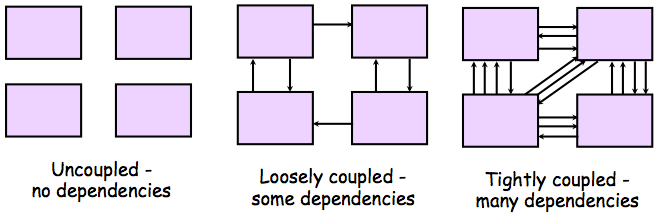
\includegraphics[width=0.5\linewidth]{coupling.png}
\end{figure}


\begin{tabular}{m{11cm}m{7cm}}
There are different types of coupling (worse to best order):
\begin{itemize}
    \item \textbf{Content coupling}: A branch into the code of B, method invocation
    \item \textbf{Common coupling }: A and B share common data, public variable
    \item \textbf{Control coupling}: A controls the behaviour of B by passing information of what to do.
    \item \textbf{Stamp coupling  }: A pass data structure to B, they have to agree on data format
    \item \textbf{Data coupling   }: A pass simple data to B, only necessary data, an integer via parameter
\end{itemize}
&
    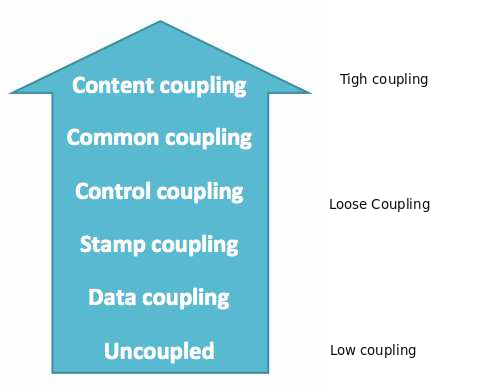
\includegraphics[width=0.8\linewidth]{types_of_coupling.png}
\end{tabular}


\subsubsection{Cohesion}

The dependence among a module's internal elements (the more, the better). 

\begin{tabular}{m{11cm}m{7cm}}
Different types of cohesion (worst to best order):
\begin{itemize}
\item \textbf{Coincidental     }: parts are unrelated
\item \textbf{Logical          }: parts related by the logic structure of the code (eg. Common code but unrelated functions)
\item \textbf{Temporal         }: parts are used in the same time in an execution
\item \textbf{Procedural       }: parts belong to a common procedure (temporal + common purpose)
\item \textbf{Communication    }: parts operate on the same data set
\item \textbf{Functional (best)}: all and only parts essential to a single function
\item \textbf{Informational    }: all and only parts essential to a single abstraction
\end{itemize}
&
    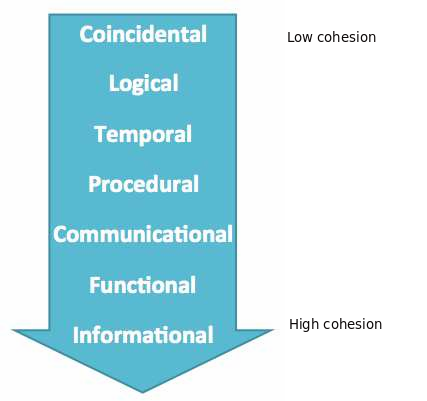
\includegraphics[width=0.8\linewidth]{types_of_cohesion.png}
\end{tabular}


\subsection{Incremental development based on the use graph}

The goal is to implement and test incrementally (i.e.\ identify progressively larger sets of
units). To do that, we need to know the dependencies between units $\rightarrow$ use graph.

\paragraph{Use Relation} A uses B iff A requires the presence of B to complete its task.

 
\begin{figure}[!ht]
    \begin{minipage}{\linewidth}
        \begin{minipage}{0.45\linewidth}
            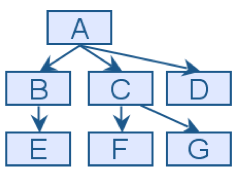
\includegraphics[width=0.6\linewidth]{use_graph_1.png}
        \end{minipage}
        \begin{minipage}{0.45\linewidth}
            Nodes = software units \newline
            Edges = \enquote{uses}
        \end{minipage}
    \end{minipage}
\end{figure}

\begin{itemize}
\item Fan-in: the number of units that use a particular unit. 
\item Fan-out: the number of units used by a particular unit. 
\item[$\Rightarrow$] Goal: high fan-in, low fan-out.
\end{itemize}

Cycles in uses graph = mutual dependency $\rightarrow$ Sandwiching: decomposing a unit into two units

\begin{figure}[!ht]
    \centering
    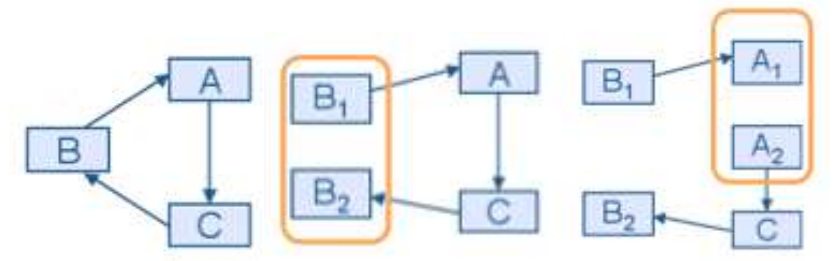
\includegraphics[width=0.6\linewidth]{use_graph_2.png}
\end{figure}

\subsection{Information hiding}

Each design decision is hidden inside a software unit = encapsulation.
\begin{itemize}
    \item Information hiding helps cohesion (hide data representation, hide an algorithm)
    \item and reduce coupling.
\end{itemize}

In OO design, an object is abstract type that hides data representation.
\textbf{Objects cannot be totally uncoupled} (need to know the identity of other
objects to invoke $\Rightarrow$ unavoidable when accessing specific
objects, but avoidable for arbitrary object (e.g: in a pool))

\subsection{Abstraction}

Omitting some details (e.g.\ pseudo-code vs.\ full code (with some non-pertinent aspect about the algorithm)). 

Different kinds of details:
\begin{itemize}
\item Decomposition hierarchy $\Rightarrow$ abstract from internal structure
\item Interface specification $\Rightarrow$ abstract from internal design details
\item Architectural views $\Rightarrow$ abstract on one particular aspect
\item Virtual machine (layer) $\Rightarrow$ abstract from lower level machine (layer)
\end{itemize}

\subsubsection{Example}
\begin{itemize}
    \item High level:

\begin{lstlisting}
sort L in nondecreasing order
\end{lstlisting}

    \item low level:

\begin{lstlisting}
DO WHILE i is between 1 and (length of L)-1:
    set LOW to
        index of smallest value in L(i),...,K(length L)
    Interchange L(i) and L(LOW)
ENDDO
\end{lstlisting}
\end{itemize}

\subsection{Generality}

Make a software unit as universally applicable as possible (increase
reusability).

Several ways of doing this:

\begin{itemize}
\item Parameterizing context-specific information $\Rightarrow$ reuse by changing parameters
instead of code
\item Removing pre-conditions $\Rightarrow$ less conditions for reuse
\item Simplifying post-conditions $\Rightarrow$ decompose into simpler units, more broadly reusable
\end{itemize}
